%\documentclass[11pt, oneside]{article}  
%\lfoot{Enzia Schnyder} %your name in the footer

% Note: Packages are already included at the top in global_handouts.tex
%\usepackage{style-3yp} %this is the .sty file
%\usepackage{pdflscape}
%\usepackage{float}
%\usepackage{longtable}
%table
%\usepackage{array}
%\newcolumntype{L}{>{\centering\arraybackslash}m{2.5cm}}
%\newcolumntype{J}{>{\centering\arraybackslash}m{4.1cm}}
%\newcolumntype{M}{>{\centering\arraybackslash}m{5cm}}
%\newcolumntype{N}{>{\centering\arraybackslash}m{3.5cm}}
%\usepackage{multirow}
%\usepackage{gensymb} %degrees symbol
%\usepackage [version=4] {mhchem}

%\begin{document}
\section{Heat Exchange Network}
\begin{figure} [h]
\centering
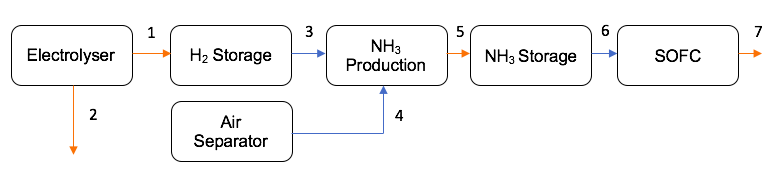
\includegraphics[width=0.9\textwidth]{./pictures/heatexflow.png}
  \caption{A diagram showing how different streams in the heat exchange network are related to the process units. Blue arrows represent cold streams that must be heated up and red arrows represent hot streams that must be cooled} \label{fig:heatexflow}
\end{figure}

\begin{table} [h]
\begin{center}
\caption{Data for streams coming in and out of all major process units of the ESS plant} \label{tab:heatexdata} 
\begin{tabular}{ |c|c|L|c|c|c|L| }
 \hline
Stream & Composition & $\dot{m} $ $(kg/s) $& $C_p$ $(kJ kg^{-1} K^{-1})$  & $T_{in}$ $(K)$ & $T_{out}$ $(K)$ & $\Delta H$ $(kW)$ \\ 
 \hline
  1 & $H_2$ & 0.4844 & 14.3 & 393 & 298 & -658\\ 
 \hline
 2 & $O_2$ & 35.75 & 0.919 & 393 & 298 & -3119\\ 
 \hline
3 & $H_2$ & 0.5099 & 14.3 & 298 & 473 & 1276\\
\hline
4 & $N_2$ & 2.34 & 1.04 & 288 & 473 & 450.2\\
 \hline
  5 & $NH_3$ & 2.795 & 2.19 & 238 & 233 &-30.6\\
 \hline
 6 & $NH_3$ & 2.655 & 2.19 & 233 & 243 & 58.1\\
 \hline
 7 & Air & 200 & 1.01 & 898 & 298 & -121200\\
 \hline
\end{tabular}
\end{center}  
\end{table}

\begin{figure} [H]
\centering
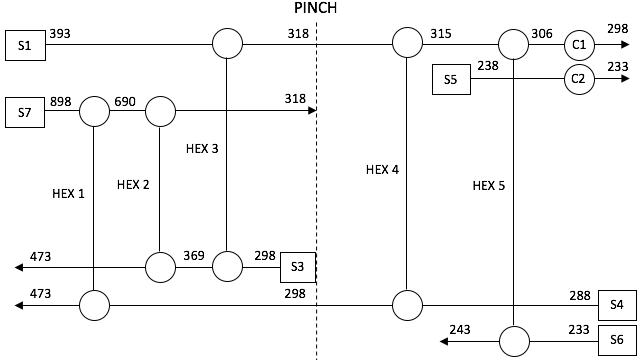
\includegraphics[width=0.72\textwidth]{./pictures/heatexnetworkBIG.png}
  \caption{The final heat exchange network. Horizontal lines represent streams, each pair of circles represents a heat exchanger, single circles represent cooling utility and temperatures (K) are shown at each isothermal segment.} \label{fig:heatexnetwork}
  \end{figure}

\begin {table} [h]
\begin{center}
\caption{Heat transferred in all heat exchangers and utilities in the network} \label{tab:powerhex} 
\begin{tabular}{ |c|c|c|c|c|c|c|c|c| }
 \hline
\multirow{2}{*}{Component} & \multicolumn{5}{|c|}{Heat exchangers}& \multicolumn{2}{|c|}{Cooling Utilities}\\ 
 \cline{2-8}
   & HEX 1 & HEX 2 & HEX 3 & HEX 4 &HEX 5 & C1 & C2\\ 
 \hline
 Enthalpy change (kW) & 425.3 & 756.0 & 519.8 & 24.3 & 58.1 & 56.2 & 30.6\\ 
 \hline
\end{tabular}
\end{center}  
\end {table}

%\end{document}